%-----------------------------------------------------------------------
% 
%-----------------------------------------------------------------------
%
%     
%
%
%%%%%%%%%%%%%%%%%%%%%%%%%%%%%%%%%%%%%%%%%%%%%%%%%%%%%%%%%%%%%%%%%%%%%%%%


\documentclass[twoside]{article}
\usepackage{amsmath,amsthm,amssymb,verbatim}

%     If your article includes graphics, uncomment this command.
\usepackage{graphicx}

%     If the article includes commutative diagrams, ...
%\usepackage[cmtip,all]{xy}

\usepackage{url}

\usepackage{fancyhdr}
\usepackage{hyperref}
\pagestyle{fancy}

\def\blfootnote{\xdef\@thefnmark{}\@footnotetext} 
\long\def\symbolfootnote[#1]#2{\begingroup%
\def\thefootnote{\fnsymbol{footnote}}\footnote[#1]{#2}\endgroup} 

	\addtolength{\oddsidemargin}{1cm}
	\addtolength{\evensidemargin}{-1cm}

\setcounter{page}{1}

\begin{document}

%     If you need symbols beyond the basic set, uncomment this command.
%\usepackage{amssymb}


\newtheorem{theorem}{Theorem}[section]
\newtheorem{lemma}[theorem]{Lemma}

\theoremstyle{definition}
\newtheorem{definition}[theorem]{Definition}
\newtheorem{example}[theorem]{Example}
\newtheorem{xca}[theorem]{Exercise}

\theoremstyle{remark}
\newtheorem{remark}[theorem]{Remark}

\numberwithin{equation}{section}


\date{}
\lhead[]{}
\chead[\underline{Generative AI}]{\it{O. Shanker}}
\rhead[]{}

% \title[short text for running head]{full title}
\title{\bf{Generative AI predicts the Riemann zeta zero distribution}}

\maketitle


%    author one information
% \author[short version for running head]{name for top of paper}
\author{{\textbf{O. Shanker}},}
\thanks{ Mountain View, CA 94041, U. S. A. email: oshanker@gmail.com}

\thispagestyle{fancy}

%    Abstract is required.
\begin{abstract}
Abstract. 
The Transformer architecture of Generative AI is very successful in predicting the distribution of Riemann zeta zero counts on consecutive Gram intervals. We get accuracies of $0.998$
in predicting a sequence of ten consecutive zero counts. We tested with two ranges of Riemann zeta zeros, $t=10^{12}$ and $t=10^{28}$. With special training for rare events, we can get essentially full prediction. This shows that applying the technique to more complex problems has great promise. We have used very minimal computer resources compared to typical models in language applications. With access to better resources, we can attack much more important problems.
DOI: \href{http://dx.doi.org/10.36227/techrxiv.171822467.73136863/v1}{10.36227/techrxiv.171822467.73136863/v1}

\end{abstract}
{\textbf {Keywords}:} COMPUTING AND PROCESSING, Generative AI, Riemann zeta, Zero Distribution,  Transformer Architecture 


\symbolfootnote[0]{Generative AI has more applications than you imagine!}


\section{Introduction}

 Machine Learning applications have been used in the literature in the study of the Riemann zeta zeros \cite{osneural,Shanker 2018a,osentropy}.
Why use machine learning  as a tool to the study of the behaviour of the Riemann zeta function?  Machine Learning is a great tool which can extract patterns when one has a huge amount of data and one does not have a complete human understanding of the patterns underlying the phenomenon being studied. With tens of trillions of the Riemann zeta function having been evaluated, one has the huge data set which would enable the application of machine learning techniques. Another indication that machine learning will be useful is a study of the entropy of the Riemann zeta zeros~\cite{osentropy}, which shows that the pattern of zeros shows a good amount of order. In this study we apply Generative AI to predict the sequence of zero counts on Gram intervals. The problem we are solving is, given a set of ten consecutive zero counts on Gram intervals, predict the next set of ten consecutive zero counts. This is a simple problem. If we can model this well, it open up the possibilities for attacking more complex problems. In Table~\ref{tab:sequence} we show a sequence of zero counts on consecutive Gram intervals. The sequence of counts has been broken up into separate rows, merely for convenience in presentation. For those who do not wish to get too deep into Riemann zeta theory, just ignore all the discussion about the theory, and understand that we have a sequence of counts, and we wish to see how well Generative AI does in predicting the pattern underlying the sequence of counts. This is a precursor to further applications. This is a continuation of preliminary work reported in Ref.~\cite{osgenai}.


\section{\label{sec2}Materials and Methods}
We describe the problem domain and our model.

\subsection{\label{seckaratsuba}Riemann zeta zero counts on Gram Intervals}

In this section we consider the distribution of Gram intervals that contain a given number of zeros. 
\begin{table}
\centering \(\begin{array}{ccccccccccccccc}
\hline
2& 0& 1& 2& 0& 1& 1& 1& 0& 2& 1& 0& 1& 2& 1 \\
2& 0& 1& 1& 1& 2& 0& 1& 1& 1& 0& 2& 1& 1& 1 \\
0& 2& 1& 2& 1& 0& 1& 1& 1& 1& 1& 1& 1& 1& 1 \\
1& 1& 1& 1& 1& 1& 1& 0& 1& 2& 1& 1& 1& 1& 0 \\
2& 1& 1& 0& 3& 1& 0& 2& 1& 1& 0& 1& 1& 1& 1 \\
\hline
\end{array}\)
\caption{Count of zeros on consecutive Gram intervals (shown on multiple lines for convenience).} 
\label{tab:sequence}
\end{table}

 Odlyzko~\cite{Odlyzko 1992} made a conjecture regarding the distribution of Gram intervals that contain a given number of zeros. The conjecture is that at large heights a Gram interval does not differ from any other interval of that length. Odlyzko used this conjecture, and the GUE hypothesis, to derive the distribution of Gram intervals that contain a given number of zeros.  
The GUE hypothesis  is the hypothesis that the distribution of the normalized spacing between zeros of the Zeta function is asymptotically equal to the distribution of the eigenvalues of random hermitian matrices with independent normal distribution of its coefficients. With these assumptions the distribution of Gram intervals that contain a given number of zeros is given by the probability that an interval of length equal to the Gram interval contains exactly $m$ zeros. 

Table~\ref{tab:intervalzeros} shows the counts of Gram intervals that contain $m$ zeros, for a sample at heights  $t=10^{12}$ and $t=10^{28}$, and the  expected values for the counts from Odlyzko's prediction. Further discussion about the topic can be found in Ref~\cite{Shanker 2018a}. We use the zeros from Ref~\cite{hiary 2010}. The last row is from Table 2.13.3 of Ref.~\cite{Odlyzko 1992}. The agreement with Odlyzko's prediction is very good. 


\begin{table}
\centering \(\begin{array}{lllll}\\
\hline
 &count = 0&count = 1&count = 2&count = 3\\
\hline
t = 10^{12}&0.14880&0.70440&0.14482&0.00199\\
t = 10^{28}&0.16192&0.67815&0.15795&0.00199\\
Odlyzko&0.17022&0.66143&0.16640&0.00186\\
\hline
\end{array}\)
\caption{Distribution of Gram intervals that contain $m$ zeros at  $t=10^{12}$.} 
\label{tab:intervalzeros}
\end{table}


\subsection{\label{secwhy}Why Machine Learning?}

At large heights evaluating the Riemann zeta function  is a non-trivial task, requiring much computer time 
and knowledge of special techniques.  It would be useful to apply
machine learning~\cite{osneural,Shanker 2018a}
as a guide to identify the T values where we can expect to see behaviour of interest.

We use PyTorch~\cite{pytorch} as the python framework to perform the machine learning 
task. We use the Transformer Architecture~\cite{vaswani} which is widely used in Generative AI. 

The key concept underlying the advances in Natural Language Processing (NLP) is Attention. In Attention when the model is predicting the next word it searches for a set of positions in the source sentence where the most relevant information is concentrated. 
Consider the sentence "Amidst the cacophony of bustling city streets, where the relentless symphony of car horns blares incessantly, echoing through the labyrinthine alleyways adorned with vibrant graffiti, there lies a quaint cafe nestled in a quiet corner, its cozy interior exuding an inviting warmth that beckons weary souls seeking solace from the frenetic pace of urban life". The "cacophony" and "quaint cafe" are separated in position, however, they are closely related and the relation is important to understand the sentence. The Attention concept brings out this interacton.

Earlier models in NLP used for sequence-to-sequence learning relied on Recurrent Neural Networks which are computationnally expensive. They had to process sequences step by step, whereas Transformers only need to look once at the whole sequence, moving the time complexity from O(n) to O(1). The Transformer lends itself to parallelization. 
Regarding the feature set, 
Ref~\cite{osneural,Shanker 2018a} found that the behavior of the zeta function at Gram points 
is a good starting point to extract features for use in prediction. 
Related  results can be found in Ref.~\cite{oscue, os6, Shanker 2018b,Shanker 2020}. We therefore
use as our feature set for prediction the distribution of zero counts on Gram Intervals.



\begin{figure*}
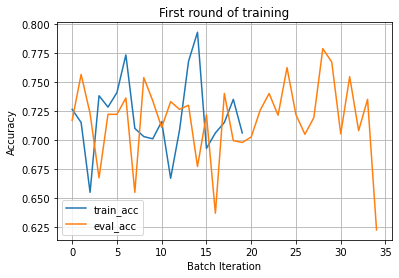
\includegraphics[width=1.0\textwidth]{Round1.png}
\caption[]{ 
 Training and validation accuracies during Round 1 ($t=10^{12}$).
 }
\vspace{1mm}, 
\label{fig:round1}
\end{figure*}


\begin{figure*}
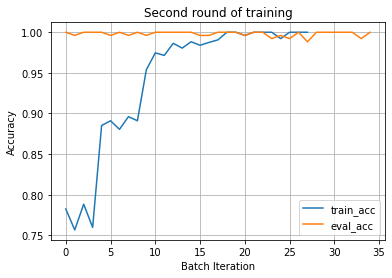
\includegraphics[width=1.0\textwidth]{Round2.png}
\caption[]{ 
 Training and validation accuracies during Round 2 ($t=10^{12}$).
 }
\vspace{1mm}, 
\label{fig:round2}
\end{figure*}




\subsection{\label{sec3.1} Choosing the Model}
Typical applications of Transformers involve use of huge amounts of computing resources and data to learn, for example, Natural Language processing. Here, we extend the application to a mathematical domain, the Riemann Zeta function. Since this is a new domain of application, we build a very simple model to study how well the simple model performs. For the Transformer model we build upon the presentation in  Ref~\cite{BenjaminEtienne}. The code for our implementation is available at 
 Ref~\cite{shankergit}.


\begin{table}
\centering \(\begin{array}{ccc}
\hline
\hline
Training  & Training &Validation  \\
set     &accuracy&accuracy\\
\hline
1  & 0.675 & 0.716 \\

2  & 0.914 & 0.998 \\
\hline
\end{array}\)
\caption{Training and validation accuracies $t=10^{12}$}
\label{tab:accuracies12}
\end{table}

\subsubsection{\label{10E12} $t=10^{12}$}
We use the Transformer implementation of Ref~\cite{shankergit} to do two rounds of training and validation. In the first round we use $6400$ samples for training, and $10000$ samples for validation. Figure~\ref{fig:round1} shows the training and validation accuracies, after each batch of 256 samples is used for training. Thus, with $6400$ samples we have 25 batches. In the figure we don't show the first 5 batches, since the initial training runs obviously will be noisy (until the model learns the pattern at least roughly). We validated with $10000$ samples. The average training and validation accuracies are $0.675$ and $0.716$ respectively (Table~\ref{tab:accuracies12}).

In the second round we use $8400$ samples for training, and $10000$ samples for validation. Figure~\ref{fig:round2} shows the training and validation accuracies, after each batch of 256 samples is used for training.  We validated with $10000$ samples. The average training and validation accuracies are $0.914$ and $0.998$ respectively. Since the second round of training uses the model trained on the first round, the accuracy is higher.



\begin{figure*}
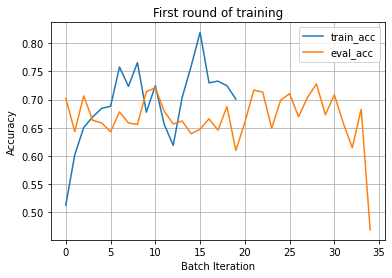
\includegraphics[width=1.0\textwidth]{Round1_28.png}
\caption[]{ 
 Training and validation accuracies during Round 1 ($t=10^{28}$).
 }
\vspace{1mm}, 
\label{fig:round1_28}
\end{figure*}


\begin{figure*}
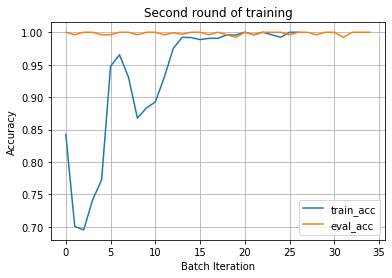
\includegraphics[width=1.0\textwidth]{Round2_28.png}
\caption[]{ 
 Training and validation accuracies during Round 2 ($t=10^{28}$).
 }
\vspace{1mm}, 
\label{fig:round2_28}
\end{figure*}

\subsubsection{\label{10E28} $t=10^{28}$}

We also studied the range of zeros at $t=10^{28}$ and get similar results. We  do two rounds of training and validation. In the first round we use $6400$ samples for training, and $10000$ samples for validation. Figure~\ref{fig:round1_28} shows the training and validation accuracies, after each batch of 256 samples is used for training.  We validated with $10000$ samples. The average training and validation accuracies are $0.648$ and $0.669$ respectively (Table~\ref{tab:accuracies28}).

In the second round we use $8400$ samples for training, and $10000$ samples for validation. Figure~\ref{fig:round2_28} shows the training and validation accuracies, after each batch of 256 samples is used for training.  We validated with $10000$ samples. The average training and validation accuracies are $0.902$ and $0.999$ respectively. Since the second round of training uses the model trained on the first round, the accuracy is higher.


\begin{table}
\centering \(\begin{array}{ccc}
\hline
\hline
Training  & Training &Validation  \\
set     &accuracy&accuracy\\
\hline
1  & 0.648 & 0.669 \\

2  & 0.902 & 0.999 \\
\hline
\end{array}\)
\caption{Training and validation accuracies $t=10^{28}$}
\label{tab:accuracies28}
\end{table}

\subsection{\label{relation}Training,  Model predictions}

Table~\ref{tab:accuracies12} and Table~\ref{tab:accuracies28} show the model accuracy during training and validation phases, for two rounds of training, for $t=10^{12}$ and $t=10^{28}$ respectively. Since the second round of training uses the model trained on the first round, the accuracy is higher. The final validation accuracy is 0.998 for a validation sample size of $10000$. The $0.998$ comes from the fact that the counts of Gram intervals that contain $3$ zeros or more zeros is rare (Table~\ref{tab:intervalzeros}). The model will not learn the patterns with large zero counts very well. 
Table~\ref{tab:perf} shows the prediction for the next set of ten consecutive zero counts, given a set of ten consecutive zero counts on Gram intervals.  

\begin{table}
\centering \(\begin{array}{ccccccccccc}
\hline
Counts& \\
\hline
actual     &1&1&1&1&1&1&1&1&0&1\\
prediction &1&1&1&1&1&1&1&1&0&1\\
\hline
actual     &1&1&1&1&1&1&1&0&1&1\\
prediction &1&1&1&1&1&1&1&0&1&1\\
\hline
actual     &1&1&1&1&1&1&0&1&1&2\\
prediction &1&1&1&1&1&1&0&1&1&2\\
\hline
actual     &1&1&1&1&1&0&1&1&2&1\\
prediction &1&1&1&1&1&0&1&1&2&1\\
\hline
actual     &1&1&1&1&0&1&1&2&1&0\\
prediction &1&1&1&1&0&1&1&2&1&0\\
\hline
\end{array}\)
\caption{Comparison of model prediction for zero counts with actuals, for different sequences of $10$ Gram intervals} 
\label{tab:perf}
\end{table}

\subsection{\label{rarefix}Fixing the model for rare events}
The accuracy of $0.998$ is due to the presence of rare events where the Gram interval contains $3$ or more zeros. To handle this situation, we cull samples containing such rare events from a set of $10$ million zeros at $t=10^{28}$. From the $10$ million zeros we were able to get a sample of $19616$ rare events. When we pre-train the model with this set, and then train the model on the given dataset, we get essentially completely accurate predictions.


\section{\label{conclusions}Conclusions}
The Transformer architecture of Generative AI is very successful in predicting the distribution of Riemann zeta zero counts on consecutive Gram intervals. Without special treatment we get accuracies of $0.998$
in predicting a sequence of ten consecutive zero counts. When we pre-train the model with a set of rare events, and then train the model on the given dataset, we get essentially completely accurate predictions.
 This shows that applying the technique to more complex problems has great promise. 

We have used very minimal computer resources compared to typical models in language applications. With access to better resources, we can attack much more important problems.

\section*{Acknowledgments and Funding Statement}

 The study was done as an independent researcher. There was no
external funding.



\bibliographystyle{amsplain}
\begin{thebibliography}{10}

\bibitem{osneural} O. Shanker, ``Neural Network prediction of Riemann zeta zeros''
{\it Advanced Modeling and Optimization}, {\bf 14}, 717-728, (2012), \url{https://www.researchgate.net/publication/273945970_Neural_Network_prediction_of_Riemann_zeta_zeros}.


\bibitem{Shanker 2018a} O. Shanker, 
``Good to Bad Gram Point Ratio For Riemann Zeta Function",
{\it Experimental Mathematics} {\bf 30}, 76-85,
\url{https://doi.org/10.1080/10586458.2018.1492474}(2021)

\bibitem{osentropy} O. Shanker, ``Entropy of Riemann zeta zero sequence''
{\it Advanced Modeling and Optimization}, {\bf 13}, 449-456, (2013). 

\bibitem{osgenai} O. Shanker, 
``Can Generative AI understand the Riemann zeta zero distribution?'',
 Researchgate report DOI: 10.13140/RG.2.2.34678.00323/1,
\url{https://tinyurl.com/3vx5uvte}, 
(2024). 

\bibitem{Odlyzko 1992}  A. Odlyzko,
``The $10^{20}$-th Zero of the Riemann Zeta
Function and 175 Million of its Neighbors", report,
\url{http://www.dtc.umn.edu/~odlyzko/unpublished/zeta.10to20.1992.pdf}, (1992)

\bibitem{hiary 2010} G. A. Hiary,
``An amortized-complexity method to compute the Riemann zeta function", 
{\it Mathematics of Computation} {\bf80}(2011), 1785-1796


\bibitem{pytorch} Paszke, Adam and Gross, Sam and Chintala, Soumith and Chanan, Gregory and Yang, Edward and DeVito, Zachary and Lin, Zeming and Desmaison, Alban and Antiga, Luca and Lerer, Adam, 
``Automatic differentiation in PyTorch'',
 NIPS 2017 Workshop Autodiff Proceedings,
\url{https://openreview.net/pdf?id=BJJsrmfCZ}, 
(2017). 

\bibitem{vaswani} Vaswani, A., Shazeer, N., Parmar, N., et al. 
``Attention is All you Need.'', 
Advances in Neural Information Processing Systems 30: Annual Conference                    on Neural Information Processing Systems 2017, December 4-9, 2017,  Long Beach, CA, USA, 5998--6008.

\bibitem{oscue} O. Shanker, 
``Random Matrix Theory explanation for Riemann Zeta Value Distribution Symmetry'',
 Researchgate report DOI 10.13140/RG.2.2.20155.39209,
\url{http://dx.doi.org/10.13140/RG.2.2.20155.39209}, 
(2022). 


\bibitem{os6} O. Shanker, 
``Generalised Zeta Functions and Self-Similarity of Zero Distributions",
{\it J.  Phys. A} {\bf39}(2006), 13983-13997

\bibitem{Shanker 2018b} O. Shanker, 
``Symmetry properties of distribution of Riemann Zeta Function values on critical axis'',
 Researchgate report DOI 10.13140/RG.2.2.34433.35687,
\url{http://dx.doi.org/10.13140/RG.2.2.34433.35687}, 
(2018). 

\bibitem{Shanker 2020} O. Shanker, 
``Universality of Riemann Zeta Function value distribution on critical axis'',
 Researchgate report DOI 10.13140/RG.2.2.18693.29927,
\url{http://dx.doi.org/10.13140/RG.2.2.18693.29927}, 
(2020). 

\bibitem{BenjaminEtienne} Benjamin Etienne, 
``A Complete Guide to Write your own Transformers'',
 Towards Data Science,
\url{https://tinyurl.com/3wur9tux}, 
(2024). 

\bibitem{shankergit} O. Shanker, 
Source code on github,
\url{https://tinyurl.com/9yura82b}, 
(2024). 



\end{thebibliography} 

\end{document}
